%-----------------------------------------------------------------
\section{Daughter boards}
\label{sec:daughter}
%-----------------------------------------------------------------
A FLEX Daughter Board is a board with specialized features that can be added on top of a FLEX Base Board, refer Section  ~\ref{sec:base} (by piggybacking, refer Figure ~\ref{fig:piggyback}), to obtain complex devices for all possible applications.\\

\noindent Evidence Srl and Embedded Solutions propose a set of general purpose Daughter Boards for some of the most common applications.\\

\noindent The development of customised, refer Section ~\ref{sec:custom}, or home-made Daughter Boards are made easy as the FLEX Base Board connectors uses the standard 2.54mm pitch. Hence, virtually, the extending of features of the FLEX platform, refer Table ~\ref{tbl:base}, is unlimited.



%+-+-+-+-+-+-+-+-+-+-+-+-+-+-+-+-+-+-+-+-+-+-+-+-+-+-+-+-+-+-+-+-+
\subsection{[FLEX100] FLEX Thru Hole Daughter Board}
\label{subsec:100}
%+-+-+-+-+-+-+-+-+-+-+-+-+-+-+-+-+-+-+-+-+-+-+-+-+-+-+-+-+-+-+-+-+
The board, depicted in Figure ~\ref{fig:100}, is targeted for the development of small, homemade, custom circuits that can be transparently interfaced with the FLEX Base Boards, refer Figure ~\ref{fig:base}.\\

\begin{figure}[!ht]
	\centering
		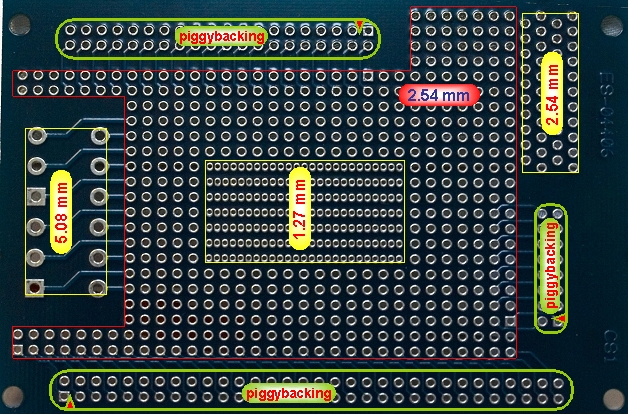
\includegraphics[width=0.90\textwidth,bb=0 0 629 415]{images/flex100.jpg}
	\caption{[FLEX100] FLEX Thru Hole Daughter Board}
	\label{fig:100}
\end{figure}

\noindent The board makes available to the user several common pinholes for connecting electronic components. Pinholes marked with "piggybacking" are pins which come from the piggybacked FLEX board, refer Figure ~\ref{fig:piggyback}, and each pin on the piggybacking row is connected to a pin on the most wide board section.\\


%^^^^^^^^^^^^^^^^^^^^^^^^^^^^^^^^^^^^^^^^^^^^^^^^^^
\subsubsection{Technical details}
\label{subsubsec:100tech}
%^^^^^^^^^^^^^^^^^^^^^^^^^^^^^^^^^^^^^^^^^^^^^^^^^^
\begin{small}
\begin{table}[!ht]
\centering
\begin{tabular}{|l|}
  \hline
  $\bullet$ \hspace{0.1cm} {\tt CON3:} 16 pin connector, refer Table ~\ref{tbl:con3}\\
  $\bullet$ \hspace{0.1cm} {\tt CON5:} 40 pin connector, refer Table ~\ref{tbl:con5}\\
  $\bullet$ \hspace{0.1cm} {\tt CON6:} 64 pin connector, refer Table ~\ref{tbl:con6}\\
  \hline
\end{tabular}
\caption{FLEX100 - Standard Connectors for Piggybacking}
\label{tbl:100piggy}
\end{table}
\end{small}

\begin{small}
\begin{table}[!ht]
\centering
\begin{tabular}{|l|}
  \hline
  $\bullet$ \hspace{0.1cm} 5.08 mm for clamps\\
  $\bullet$ \hspace{0.1cm} 2.54 mm for RJ45, RS232, etc. connectors\\
  $\bullet$ \hspace{0.1cm} 2.54 mm for all other components\\
  $\bullet$ \hspace{0.1cm} 1.27 mm for typical SMD components\\
  \hline
\end{tabular}
\caption{FLEX100 - Standard Pinhole Patterns}
\label{tbl:100pattern}
\end{table}
\end{small}



%+-+-+-+-+-+-+-+-+-+-+-+-+-+-+-+-+-+-+-+-+-+-+-+-+-+-+-+-+-+-+-+-+
\clearpage
\subsection{[FLEX101] FLEX Multibus Base Daughter Board}
\label{subsec:101}
%+-+-+-+-+-+-+-+-+-+-+-+-+-+-+-+-+-+-+-+-+-+-+-+-+-+-+-+-+-+-+-+-+
The FLEX Multibus Base Board, as depicted in Figure ~\ref{fig:101}, is a FLEX Daughter Board, refer Section ~\ref{sec:daughter}. It fits directly on FLEX Base Board (FLEX Full, refer Subsection ~\ref{subsec:001}/FLEX Light, refer Subsection ~\ref{subsec:003}), and number of slots, refer Table ~\ref{tbl:101slots}, are available for FLEX Multibus Modules to be mounted on top of it, thereby extending the FLEX platform.\\

\begin{figure}[!ht]
	\centering
		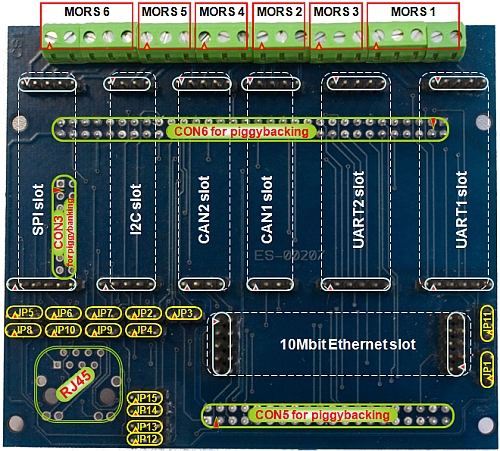
\includegraphics[width=0.90\textwidth,bb=0 0 541 500]{images/flex101.jpg}
	\caption{[FLEX101] FLEX Multibus Base Daughter Board}
	\label{fig:101}
\end{figure}
\noindent {\tt Note: The RJ45 Ethernet Connecter is not included with this product. It is sold along with the FLEX Multibus Ethernet Module, refer Subsection ~\ref{subsec:102}, and has to be soldered on the FLEX Multibus Base Daughter Board}.\\

\noindent The following slots are available on the Multibus board:
\begin{itemize}
  \item UART2 slot, for Serial TTL/RS232/RS485/RS422 module
  \item UART1 slot, for Serial TTL/RS232/RS485 module
  \item CAN1 slot, for CAN module
  \item CAN2 slot, for CAN module
  \item I2C slot (channel selectable), for I2C module
  \item SPI slot (channel selectable), for SPI module
  \item Ethernet slot, for 10Mbit Ethernet module
\end{itemize}
\noindent {\tt Note: Modules are mounted only if needed. For example, if the application requires the Ethernet interface and the connection to the CAN bus, only the corresponding modules will be mounted on the Multibus Base Board, leaving the remaining pins free for other use}.\\

\noindent {\bf Chip select of SPI Module (Slot 6):} Jumpers JP8, JP9, and JP10 control the chip select of the SPI module from either a general purpose I/O or chip select pin built-in in the microcontroller, refer Figures ~\ref{fig:101detail} and ~\ref{fig:101slot6} and Tables ~\ref{tbl:101jps} and ~\ref{tbl:107slot6_jps}.\\



%^^^^^^^^^^^^^^^^^^^^^^^^^^^^^^^^^^^^^^^^^^^^^^^^^^
\subsubsection{Technical details}
\label{subsubsec:101tech}
%^^^^^^^^^^^^^^^^^^^^^^^^^^^^^^^^^^^^^^^^^^^^^^^^^^
\begin{figure}[!ht]
	\centering
		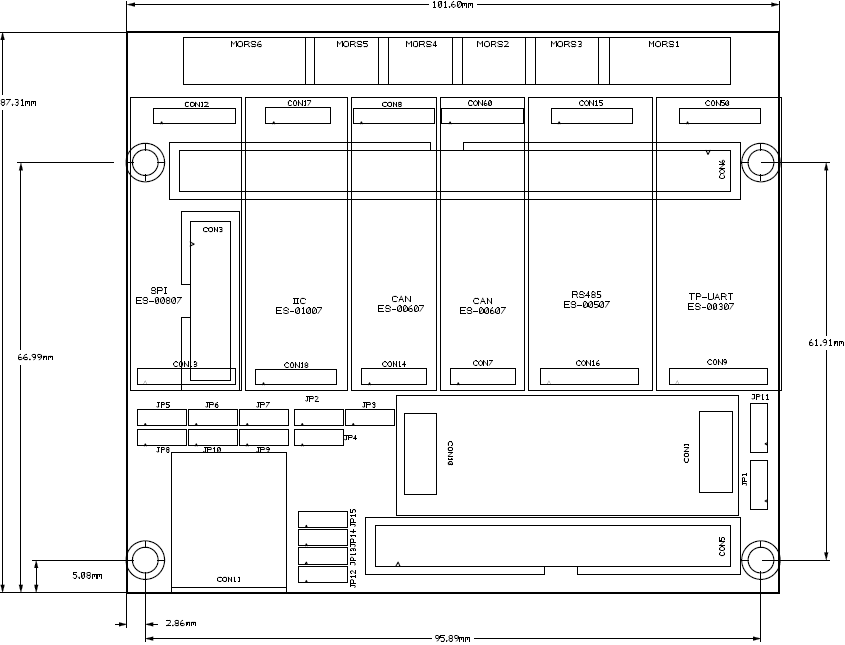
\includegraphics[width=0.90\textwidth,bb=0 0 845 645]{images/101mec.png}
	\caption{[FLEX101] Dimensions of FLEX Multibus Base Daughter Board}
	\label{fig:101mec}
\end{figure}
\begin{figure}[!ht]
	\centering
		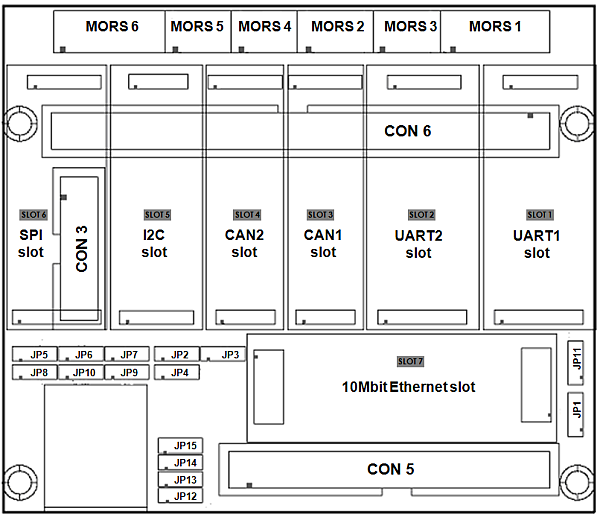
\includegraphics[width=0.90\textwidth,bb=0 0 662 589]{images/101.png}
	\caption{[FLEX101] Details of FLEX Multibus Base Daughter Board}
	\label{fig:101detail}
\end{figure}

\begin{small}
\begin{table}[!ht]
\centering
\begin{tabular}{|c|l|}
	\hline
	Pin 1 & CTS PC\\
  \hline
	Pin 2 & RX PC\\
	\hline
  Pin 3 & TX PC\\
	\hline
  Pin 4 & RTS PC\\
	\hline
  Pin 5 & GND \\
	\hline
\end{tabular}
\caption{FLEX101 - MORS1 (RS232 module)}
\label{tbl:101mors1}
\end{table}
\end{small}

\begin{small}
\begin{table}[!ht]
\centering
\begin{tabular}{|c|l|}
	\hline
	Pin 1 & O\_CAN+\\
	\hline
  Pin 2 & O\_CAN-\\
	\hline
  Pin 3 & GND\\
	\hline
\end{tabular}
\caption{FLEX101 - MORS2 (CAN1 module)}
\label{tbl:101mors2}
\end{table}
\end{small}

\begin{small}
\begin{table}[!ht]
\centering
\begin{tabular}{|c|l|}
	\hline
	Pin 1 & 485-\\
	\hline
  Pin 2 & 485+\\
	\hline
  Pin 3 & GND\\
	\hline
\end{tabular}
\caption{FLEX101 - MORS3 (RS485 module)}
\label{tbl:101mors3}
\end{table}
\end{small}

\begin{small}
\begin{table}[!ht]
\centering
\begin{tabular}{|c|l|}
	\hline
	Pin 1 & O\_CAN+1\\
	\hline
  Pin 2 & O\_CAN-1\\
	\hline
  Pin 3 & GND \\
	\hline
\end{tabular}
\caption{FLEX101 - MORS4 (CAN2 module)}
\label{tbl:101mors4}
\end{table}
\end{small}

\begin{small}
\begin{table}[!ht]
\centering
\begin{tabular}{|c|l|}
	\hline
	Pin 1 & IIC\_DIO\_C\\
	\hline
  Pin 2 & IIC\_CK\_C\\
	\hline
  Pin 3 & GND \\
	\hline
\end{tabular}
\caption{FLEX101 - MORS5 (I2C module)}
\label{tbl:101mors5}
\end{table}
\end{small}

\begin{small}
\begin{table}[!ht]
\centering
\begin{tabular}{|c|l|}
	\hline
	Pin 1 & SPI\_DO\_C\\
	\hline
  Pin 2 & SPI\_DI\_C\\
	\hline
  Pin 3 & SPI\_CLK\_C\\
	\hline
  Pin 4 & SPI\_SS\_C\\
  \hline
  Pin 5 & GND\\
	\hline
\end{tabular}
\caption{FLEX101 - MORS6 (SPI module)}
\label{tbl:101mors6}
\end{table}
\end{small}

\begin{small}
\begin{table}[!ht]
\centering
\begin{tabular}{|c|c|c|}
  \hline
  {\bf Jumper} & {\bf pos. 1-2} & {\bf pos. 2-3}\\
  \hline
	JP1 & FRCK\_1 & RESN \\
  \hline
	JP2 & IIC\_2 DIO & IIC\_1 DIO\\
	\hline
  JP3 & IIC\_2 CLK & IIC\_1 CLK\\
	\hline
  JP4 & IIC\_2 CS & IIC\_1 CS\\
	\hline
  JP5 & SPI\_2 DI & SPI\_1 DI\\
	\hline
  JP6 & SPI\_2 DO & SPI\_1 DO\\
	\hline
  JP7 & SPI\_2 CLK & SPI\_1 CLK\\
	\hline
  JP8 & SPI\_1 SS\_up & SPI\_1 SS\\
	\hline
  JP9 & SPI\_2 SS JP8/JP10 & SPI\_1 SS JP8/JP9\\
	\hline
  JP10 & SPI\_2 SS\_up & SPI\_2 SS\\
	\hline
  JP11 & GND & GND\_OUT\\
	\hline
  JP12 & LAN SPI\_2 DI & LAN SPI\_1 DI\\
	\hline
  JP13 & LAN SPI\_2 DO & LAN SPI\_1 DO\\
	\hline
  JP14 & LAN SPI\_2 CLK & LAN SPI\_1 CLK\\
	\hline
  JP15 & LAN SPI\_2 SS & LAN SPI\_1 SS\\
	\hline
  \multicolumn{3}{l}{\begin{tiny}Note: Default jumper settings are indicated by a $\bullet$\end{tiny}}\\
\end{tabular}
\caption{FLEX101 - Jumpers}
\label{tbl:101jps}
\end{table}
\end{small}

\begin{small}
\begin{table}[!ht]
\centering
\begin{tabular}{|l|}
  \hline
  $\bullet$ \hspace{0.1cm} {\tt CON3:} 16 pin piggybacking connector, refer Table ~\ref{tbl:con3} \\
  $\bullet$ \hspace{0.1cm} {\tt CON5:} 40 pin piggybacking connector, refer Table ~\ref{tbl:con5} \\
  $\bullet$ \hspace{0.1cm} {\tt CON6:} 64 pin piggybacking connector, refer Table ~\ref{tbl:con6} \\
  \hline
\end{tabular}
\caption{FLEX101 - Other Connectors}
\label{tbl:101other}
\end{table}
\end{small}


\begin{small}
\begin{table}[!ht]
\centering
\begin{tabular}{|c|c|c|c|c|c|c|}
	\hline
	{\bf Module} & {\bf Slot1} & {\bf Slot2} & {\bf Slot3} & {\bf Slot4} & {\bf Slot5} & {\bf Slot6}\\
	\hline
	RS232 (FLEX103) & $\bullet$ & $\bullet$ &  &  &  & \\
	\hline
  RS485 (FLEX104) & $\bullet$ & $\bullet$ &  &  &  & \\
	\hline
  RS422 (FLEX105) & $\bullet$ &  &  &  &  & \\
	\hline
  CAN (FLEX106) &  &  & $\bullet$ & $\bullet$ &  & \\
	\hline
  SPI (FLEX107) &  &  &  &  &  & $\bullet$ \\
	\hline
  Serial TTL (FLEX108) & $\bullet$ & $\bullet$ &  &  &  & \\
	\hline
  I2C &  &  &  &  & $\bullet$ & \\
	\hline
\end{tabular}
\caption{FLEX101 - Slot Allocation}
\label{tbl:101slots}
\end{table}
\end{small}
%|||||||||||||||||||||||||||||||||||||||||||||||||||||||||
\begin{figure}[!ht]
	\centering
		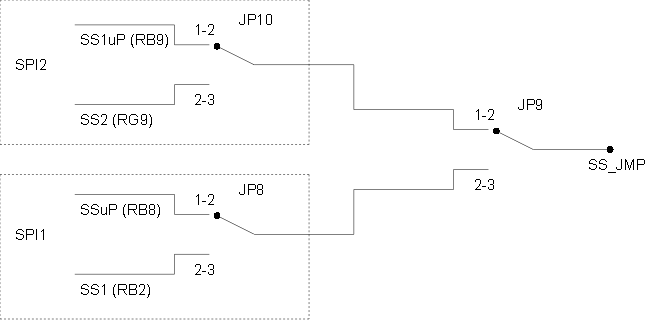
\includegraphics[width=0.50\textwidth,bb=0 0 648 320]{images/101slot6.png}
		%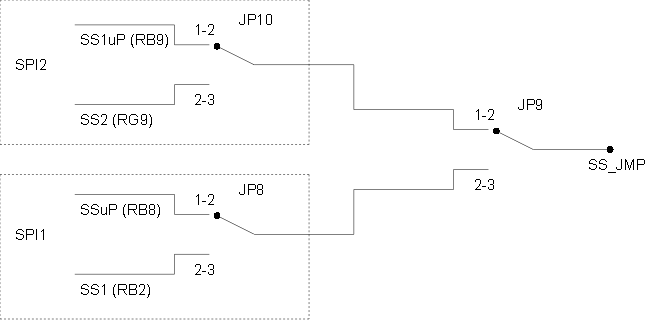
\includegraphics[width=0.50\textwidth]{images/101slot6.eps}
	\caption{[FLEX101] SPI Chip Select (Slot6) Jumper Settings}
	\label{fig:101slot6}
\end{figure}

\begin{small}
\begin{table}[!ht]
\centering
\begin{tabular}{|c|c|c|c|}
	\hline
	{\bf JP8} & {\bf JP9} & {\bf JP10} & {\bf Chip select from}\\
  \hline
   & 1-2 & 1-2 & RB9\\
	\hline
   & 1-2 & 2-3 & SS2 (RG9)\\
   \hline
  1-2 & 2-3 & & RB8\\
   \hline
  2-3 & 2-3 & & SS1 (RB2)\\
  \hline
\end{tabular}
\caption{FLEX101 - SPI Chip Select (Slot6) Jumper Settings}
\label{tbl:107slot6_jps}
\end{table}
\end{small}
%|||||||||||||||||||||||||||||||||||||||||||||||||||||||||
\clearpage
\noindent {\bf {\large Multibus Modules}}\\

\noindent The FLEX Multibus Modules are piggybacked on the FLEX Multibus Base Daughter Board, refer Subsection ~\ref{subsec:101}. These are the most widely used serial communication standards currently available: 

%+-+-+-+-+-+-+-+-+-+-+-+-+-+-+-+-+-+-+-+-+-+-+-+-+-+-+-+-+-+-+-+-+
\subsection{[FLEX102] FLEX Multibus Ethernet Module}
\label{subsec:102}
%+-+-+-+-+-+-+-+-+-+-+-+-+-+-+-+-+-+-+-+-+-+-+-+-+-+-+-+-+-+-+-+-+
The board, depicted in Figure ~\ref{fig:102}, is the Ethernet Module. It fits on slot 7 of the FLEX Multibus Base Daughter Board, refer Figure ~\ref{fig:101detail}.\\
\noindent The module can be used to export an ethernet connection through the RJ45 connector available on the Multibus Base Board. The ethernet chip used is the Microchip ENC28J60, which is connected to the dsPIC� by using the SPI bus.\\

\begin{figure}[!ht]
	\centering
		\includegraphics[width=0.50\textwidth,bb=0 0 500 200]{images/flex102.jpg}
	\caption{[FLEX102] FLEX Multibus Ethernet Module}
	\label{fig:102}
\end{figure}

\noindent {\tt Note: One RJ45 Ethernet Connecter is included with this product. It is to be soldered on the FLEX Multibus Base Daughter Board, refer Figure ~\ref{fig:101}.}\\

%^^^^^^^^^^^^^^^^^^^^^^^^^^^^^^^^^^^^^^^^^^^^^^^^^^
\subsubsection{Technical details}
\label{subsubsec:102tech}
%^^^^^^^^^^^^^^^^^^^^^^^^^^^^^^^^^^^^^^^^^^^^^^^^^^
\begin{figure}[!ht]
	\centering
		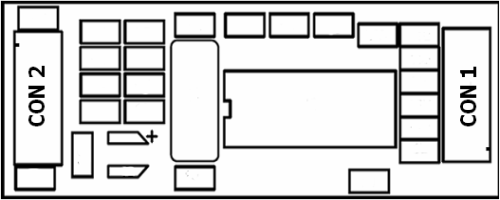
\includegraphics[width=0.50\textwidth,bb=0 0 500 200]{images/102.png}
	\caption{[FLEX102] Details of FLEX Multibus Ethernet Module}
	\label{fig:102detail}
\end{figure}

\begin{small}
\begin{table}[!ht]
\centering
\begin{tabular}{|l|l||l|l|}
	\hline
	Pin 1 & SDO\_2 & Pin 2 & SCK\_2\\
	\hline
	Pin 3 & SDI\_2 & Pin 4 & RE\_4\\
	\hline
	Pin 5 & SS\_2 & Pin 6 & INT\_4\\
	\hline
	Pin 7 & CN\_1 & Pin 8 & INT\_3\\
	\hline
	Pin 9 & GND & Pin 10 & +3.3V\\
	\hline
\end{tabular}
\caption{FLEX102 - CON1}
\label{tbl:102con1}
\end{table}
\end{small}

\begin{small}
\begin{table}[!ht]
\centering
\begin{tabular}{|l|l||l|l|}
	\hline
	Pin 1 & LED\_A & Pin 2 & TPOUT +3.3V\\
	\hline
  Pin 3 & TPOUT- & Pin 4 & TPOUT+\\
	\hline
  Pin 5 & - & Pin 6 & TPIN GND \\
	\hline
  Pin 7 & TPIN- & Pin 8 & TPIN+\\
	\hline
  Pin 9 & LED\_B & Pin 10 & GND\\
	\hline
\end{tabular}
\caption{FLEX102 - CON2}
\label{tbl:102con2}
\end{table}
\end{small}



%+-+-+-+-+-+-+-+-+-+-+-+-+-+-+-+-+-+-+-+-+-+-+-+-+-+-+-+-+-+-+-+-+
\clearpage
\subsection{[FLEX103] FLEX Multibus RS232 Module}
\label{subsec:103}
%+-+-+-+-+-+-+-+-+-+-+-+-+-+-+-+-+-+-+-+-+-+-+-+-+-+-+-+-+-+-+-+-+
The board, depicted in Figure ~\ref{fig:103}, is the Rs232 Module. It fits on slot 1 and/or slot 2 of the FLEX Multibus Base Daughter Board, refer Figure ~\ref{fig:101detail}.\\
\noindent This module can be used to export the UART pins linked to the UART peipherals on the dsPIC� by using signals which are compatible with the RS232 standard.\\

\begin{figure}[!ht]
	\centering
		\includegraphics[width=0.50\textwidth,bb=0 0 500 200]{images/flex103.jpg}
	\caption{[FLEX103] FLEX Multibus RS232 Module}
	\label{fig:103}
\end{figure}


%^^^^^^^^^^^^^^^^^^^^^^^^^^^^^^^^^^^^^^^^^^^^^^^^^^
\subsubsection{Technical details}
\label{subsubsec:103tech}
%^^^^^^^^^^^^^^^^^^^^^^^^^^^^^^^^^^^^^^^^^^^^^^^^^^
\begin{figure}[!ht]
	\centering
		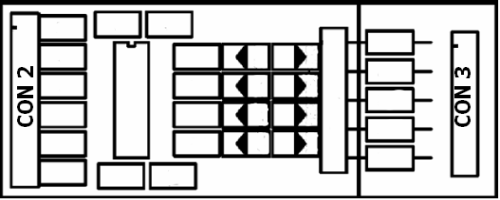
\includegraphics[width=0.50\textwidth,bb=0 0 500 200]{images/103.png}
	\caption{[FLEX103] Details of FLEX Multibus RS232 Module}
	\label{fig:103detail}
\end{figure}

\begin{small}
\begin{table}[!ht]
\centering
\begin{tabular}{|c|l|}
	\hline
	Pin 1 & +5V\\
	\hline
  Pin 2 & TX\_1\\
	\hline
  Pin 3 & SCK\_1\\
	\hline
  Pin 4 & RX\_1\\
	\hline
  Pin 5 & FRCK\_1\\
	\hline
  Pin 6 & GND\\
	\hline
\end{tabular}
\caption{FLEX103 - CON2}
\label{tbl:103con2}
\end{table}
\end{small}

\begin{small}
\begin{table}[!ht]
\centering
\begin{tabular}{|c|l|}
	\hline
	Pin 1 & CTS PC\\
	\hline
  Pin 2 & RX PC\\
	\hline
  Pin 3 & TX PC\\
	\hline
  Pin 4 & RTS PC\\
	\hline
  Pin 5 & GND\\
	\hline
\end{tabular}
\caption{FLEX103 - CON3}
\label{tbl:103con3}
\end{table}
\end{small}



%+-+-+-+-+-+-+-+-+-+-+-+-+-+-+-+-+-+-+-+-+-+-+-+-+-+-+-+-+-+-+-+-+
\clearpage
\subsection{[FLEX104] FLEX Multibus RS485 Module}
\label{subsec:104}
%+-+-+-+-+-+-+-+-+-+-+-+-+-+-+-+-+-+-+-+-+-+-+-+-+-+-+-+-+-+-+-+-+
The board, depicted in Figure ~\ref{fig:104}, is the RS485 Module. It fits on slot 1 and/or slot 2 of the FLEX Multibus Base Daughter Board, refer Figure ~\ref{fig:101detail}.\\
\noindent This module can be used to export the UART pins linked to the UART peipherals on the dsPIC� by using signals which are compatible with the RS485 standard.\\

\begin{figure}[!ht]
	\centering
		\includegraphics[width=0.50\textwidth,bb=0 0 500 200]{images/flex104.jpg}
	\caption{[FLEX104] FLEX Multibus RS485 Module}
	\label{fig:104}
\end{figure}


%^^^^^^^^^^^^^^^^^^^^^^^^^^^^^^^^^^^^^^^^^^^^^^^^^^
\subsubsection{Technical details}
\label{subsubsec:104tech}
%^^^^^^^^^^^^^^^^^^^^^^^^^^^^^^^^^^^^^^^^^^^^^^^^^^
\begin{figure}[!ht]
	\centering
		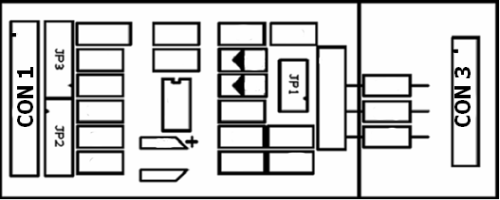
\includegraphics[width=0.50\textwidth,bb=0 0 500 200]{images/104.png}
	\caption{[FLEX104] Details of FLEX Multibus RS485 Module}
	\label{fig:104detail}
\end{figure}

\begin{small}
\begin{table} [h]
\centering
\begin{tabular}{|c|c|c|}
	\hline
	{\bf Jumper} & {\bf pos. 1-2} & {\bf pos. 2-3}\\
	\hline
	JP1 & LOOPBACK & -\\
	\hline
  JP2 & TXEN\_dsPIC & TXEN\_GND\\
	\hline
  JP3 & TXEN\_dsPIC & TXEN\_+5V\\
	\hline
  \multicolumn{3}{l}{\begin{tiny}Note: Default jumper settings are indicated by a $\bullet$\end{tiny}}\\
\end{tabular}
\caption{FLEX104 - Jumpers}
\label{tbl:104jps}
\end{table}
\end{small}

\begin{small}
\begin{table}[!ht]
\centering
\begin{tabular}{|c|l|}
	\hline
	Pin 1 & +5V\\
	\hline
  Pin 2 & TX\\
	\hline
  Pin 3 & TXEN\\
	\hline
  Pin 4 & RX\\
	\hline
  Pin 5 & -\\
	\hline
  Pin 6 & GND\\
	\hline
\end{tabular}
\caption{FLEX104 - CON1}
\label{tbl:104con1}
\end{table}
\end{small}

\begin{small}
\begin{table}[!ht]
\centering
\begin{tabular}{|c|l|}
	\hline
	Pin 1 & -\\
	\hline
  Pin 2 & RS485-\\
	\hline
  Pin 3 & RS485+\\
	\hline
  Pin 4 & -\\
	\hline
  Pin 5 & GND\\
	\hline
\end{tabular}
\caption{FLEX104 - CON3}
\label{tbl:104con3}
\end{table}
\end{small}



%+-+-+-+-+-+-+-+-+-+-+-+-+-+-+-+-+-+-+-+-+-+-+-+-+-+-+-+-+-+-+-+-+
\clearpage
\subsection{[FLEX105] FLEX Multibus RS422 Module}
\label{subsec:105}
%+-+-+-+-+-+-+-+-+-+-+-+-+-+-+-+-+-+-+-+-+-+-+-+-+-+-+-+-+-+-+-+-+
The board, depicted in Figure ~\ref{fig:105}, is the RS422 Module. It fits on slot 1 of the FLEX Multibus Base Daughter Board, refer Figure ~\ref{fig:101detail}.\\
\noindent This module can be used to export the UART pins linked to the UART peipherals on the dsPIC� by using signals which are compatible with the RS422 specification.\\

\begin{figure}[!ht]
	\centering
		\includegraphics[width=0.50\textwidth,bb=0 0 500 200]{images/flex105.jpg}
	\caption{[FLEX105] FLEX Multibus RS422 Module}
	\label{fig:105}
\end{figure}


%^^^^^^^^^^^^^^^^^^^^^^^^^^^^^^^^^^^^^^^^^^^^^^^^^^
\subsubsection{Technical details}
\label{subsubsec:105tech}
%^^^^^^^^^^^^^^^^^^^^^^^^^^^^^^^^^^^^^^^^^^^^^^^^^^
\begin{figure}[!ht]
	\centering
		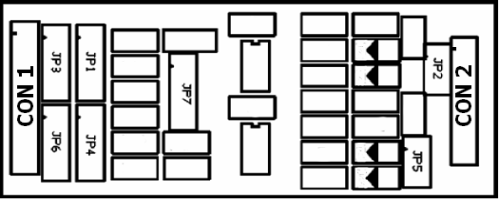
\includegraphics[width=0.50\textwidth,bb=0 0 500 200]{images/105.png}
	\caption{[FLEX105] Details of FLEX Multibus RS422 Module}
	\label{fig:105detail}
\end{figure}

\begin{small}
\begin{table}[!ht]
\centering
\begin{tabular}{|c|c|c|}
	\hline
	{\bf Jumper} & {\bf pos. 1-2} & {\bf pos. 2-3}\\
	\hline
	JP1 & TXEN\_dsPIC & TXEN +5V\\
	\hline
  JP2 & LOOPBACK\_0 & -\\
	\hline
  JP3 & TXEN\_dsPIC & TXEN GND\\
	\hline
  JP4 & TXEN\_dsPIC & TXEN +5V\\
	\hline
  JP5 & LOOPBACK\_1 & -\\
	\hline
  JP6 & TXEN\_dsPIC & TXEN GND\\
	\hline
  JP7 & RX\_0 & RX\_1\\
	\hline
  \multicolumn{3}{l}{\begin{tiny}Note: Default jumper settings are indicated by a $\bullet$\end{tiny}}\\
\end{tabular}
\caption{FLEX105 - Jumpers}
\label{tbl:105jps}
\end{table}
\end{small}

\begin{small}
\begin{table}[!ht]
\centering
\begin{tabular}{|c|l|}
	\hline
	Pin 1 & +5V\\
	\hline
  Pin 2 & TX\\
	\hline
  Pin 3 & TXEN\\
	\hline
  Pin 4 & RX\\
	\hline
  Pin 5 & -\\
	\hline
  Pin 6 & GND\\
	\hline
\end{tabular}
\caption{FLEX105 - CON1}
\label{tbl:105con1}
\end{table}
\end{small}

\begin{small}
\begin{table}[!ht]
\centering
\begin{tabular}{|c|l|}
	\hline
	Pin 1 & RS485+\_0\\
	\hline
  Pin 2 & RS485-\_0\\
	\hline
  Pin 3 & RS485+\_1\\
	\hline
  Pin 4 & RS485-\_1\\
	\hline
  Pin 5 & GND\\
	\hline
\end{tabular}
\caption{FLEX105 - CON2}
\label{tbl:105con2}
\end{table}
\end{small}



%+-+-+-+-+-+-+-+-+-+-+-+-+-+-+-+-+-+-+-+-+-+-+-+-+-+-+-+-+-+-+-+-+
\clearpage
\subsection{[FLEX106] FLEX Multibus CAN Module}
\label{subsec:106}
%+-+-+-+-+-+-+-+-+-+-+-+-+-+-+-+-+-+-+-+-+-+-+-+-+-+-+-+-+-+-+-+-+
The board, depicted in Figure ~\ref{fig:106}, is the CAN Module. It fits on slot 3 and/or slot 4 of the FLEX Multibus Base Daughter Board, refer Figure ~\ref{fig:101detail}.\\
\noindent The module can be used to export the CAN peripheral pins which are available on the dsPIC� using a CAN transceiver.\\

\begin{figure}[!ht]
	\centering
		\includegraphics[width=0.50\textwidth,bb=0 0 500 200]{images/flex106.jpg}
	\caption{[FLEX106] FLEX Multibus CAN Module}
	\label{fig:106}
\end{figure}


%^^^^^^^^^^^^^^^^^^^^^^^^^^^^^^^^^^^^^^^^^^^^^^^^^^
\subsubsection{Technical details}
\label{subsubsec:106tech}
%^^^^^^^^^^^^^^^^^^^^^^^^^^^^^^^^^^^^^^^^^^^^^^^^^^
\begin{figure}[!ht]
	\centering
		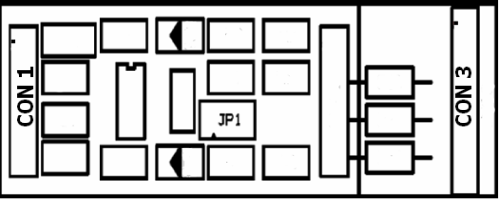
\includegraphics[width=0.50\textwidth,bb=0 0 500 200]{images/106.png}
	\caption{[FLEX106] Details of FLEX Multibus CAN Module}
	\label{fig:106detail}
\end{figure}

\begin{small}
\begin{table}[!ht]
\centering
\begin{tabular}{|c|c|c|}
	\hline
	{\bf Jumper} & {\bf pos. 1-2} & {\bf pos. 2-3}\\
	\hline
	JP1 & LOOPBACK & -\\
	\hline
  \multicolumn{3}{l}{\begin{tiny}Note: Default jumper settings are indicated by a $\bullet$\end{tiny}}\\
\end{tabular}
\caption{FLEX106 - Jumpers}
\label{tbl:106jps}
\end{table}
\end{small}

\begin{small}
\begin{table}[!ht]
\centering
\begin{tabular}{|c|l|}
	\hline
	Pin 1 & +5V\\
	\hline
  Pin 2 & RX\_CAN\\
	\hline
  Pin 3 & TX\_CAN\\
	\hline
  Pin 4 & GND\\
	\hline
\end{tabular}
\caption{FLEX106 - CON1}
\label{tbl:106con1}
\end{table}
\end{small}

\begin{small}
\begin{table}[!ht]
\centering
\begin{tabular}{|c|l|}
	\hline
	Pin 1 & -\\
	\hline
  Pin 2 & CAN+\\
	\hline
  Pin 3 & CAN-\\
	\hline
  Pin 4 & -\\
	\hline
  Pin 5 & GND\\
	\hline
\end{tabular}
\caption{FLEX106 - CON3}
\label{tbl:106con3}
\end{table}
\end{small}



%+-+-+-+-+-+-+-+-+-+-+-+-+-+-+-+-+-+-+-+-+-+-+-+-+-+-+-+-+-+-+-+-+
\clearpage
\subsection{[FLEX107] FLEX Multibus SPI Module}
\label{subsec:107}
%+-+-+-+-+-+-+-+-+-+-+-+-+-+-+-+-+-+-+-+-+-+-+-+-+-+-+-+-+-+-+-+-+
The board, depicted in Figure ~\ref{fig:107}, is the SPI Module. It fits on slot 6 of the FLEX Multibus Base Daughter Board, refer Figure ~\ref{fig:101detail}.\\
\noindent The module can be used to export one of the SPI peripheral pins which are available on the dsPIC�. The module also has a set of components which are used to protect the microcontroller pins from input signals that are not compatible with the specifications.\\

\begin{figure}[!ht]
	\centering
		\includegraphics[width=0.50\textwidth,bb=0 0 500 200]{images/flex107.jpg}
	\caption{[FLEX107] FLEX Multibus SPI Module}
	\label{fig:107}
\end{figure}


%^^^^^^^^^^^^^^^^^^^^^^^^^^^^^^^^^^^^^^^^^^^^^^^^^^
\subsubsection{Technical details}
\label{subsubsec:107tech}
%^^^^^^^^^^^^^^^^^^^^^^^^^^^^^^^^^^^^^^^^^^^^^^^^^^
\begin{figure}[!ht]
	\centering
		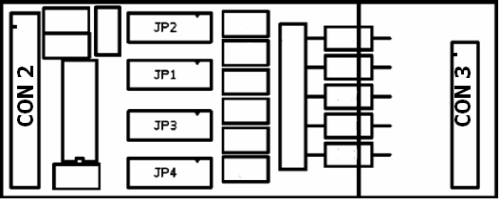
\includegraphics[width=0.50\textwidth,bb=0 0 500 200]{images/107.png}
	\caption{[FLEX107] Details of FLEX Multibus SPI Module}
	\label{fig:107detail}
\end{figure}

\begin{small}
\begin{table}[!ht]
\centering
\begin{tabular}{|c|c|c|}
	\hline
	{\bf Jumper} & {\bf pos. 1-2} & {\bf pos. 2-3}\\
	\hline
	JP1 & SPI\_DO & GND\\
	\hline
  JP2 & SPI\_CLK & GND\\
	\hline
  JP3 & SPI\_DO\_C & GND\\
	\hline
  JP4 & SPI\_SS & GND\\
	\hline
  \multicolumn{3}{l}{\begin{tiny}Note: Default jumper settings are indicated by a $\bullet$\end{tiny}}\\
\end{tabular}
\caption{FLEX107 - Jumpers}
\label{tbl:107jps}
\end{table}
\end{small}

\begin{small}
\begin{table}[!ht]
\centering
\begin{tabular}{|c|l|}
	\hline
	Pin 1 & +5V\\
	\hline
  Pin 2 & SPI\_DO\\
	\hline
  Pin 3 & SPI\_DI\\
	\hline
  Pin 4 & SPI\_CLK\\
	\hline
  Pin 5 & SPI\_SS\\
	\hline
  Pin 6 & GND\\
	\hline
\end{tabular}
\caption{FLEX107 - CON2}
\label{tbl:107con2}
\end{table}
\end{small}

\begin{small}
\begin{table}[!ht]
\centering
\begin{tabular}{|c|l|}
	\hline
	Pin 1 & SPI\_DO\_C\\
	\hline
  Pin 2 & SPI\_DI\_C\\
	\hline
  Pin 3 & SPI\_CLK\_C\\
	\hline
  Pin 4 & SPI\_SS\_C\\
	\hline
  Pin 5 & GND\\
	\hline
\end{tabular}
\caption{FLEX107 - CON3}
\label{tbl:107con3}
\end{table}
\end{small}



%+-+-+-+-+-+-+-+-+-+-+-+-+-+-+-+-+-+-+-+-+-+-+-+-+-+-+-+-+-+-+-+-+
\clearpage
\subsection{[FLEX108] FLEX Multibus Serial TTL Module}
\label{subsec:108}
%+-+-+-+-+-+-+-+-+-+-+-+-+-+-+-+-+-+-+-+-+-+-+-+-+-+-+-+-+-+-+-+-+
The board, depicted in Figure ~\ref{fig:108}, is the Serial TTL Module. It fits on slot 1 and/or slot 2 of the FLEX Multibus Base Daughter Board, refer Figure ~\ref{fig:101detail}.\\
\noindent This module can be used to export the UART pins linked to the UART peipherals on the dsPIC� by using signals which are compatible with TTL electronic equipments. The module also has a set of components which are used to protect the microcontroller pins from input signals which are not compatible with the specifications.\\

\begin{figure}[!ht]
	\centering
		\includegraphics[width=0.50\textwidth,bb=0 0 500 200]{images/flex108.jpg}
	\caption{[FLEX108] FLEX Multibus Serial TTL Module}
	\label{fig:108}
\end{figure}


%^^^^^^^^^^^^^^^^^^^^^^^^^^^^^^^^^^^^^^^^^^^^^^^^^^
\subsubsection{Technical details}
\label{subsubsec:108tech}
%^^^^^^^^^^^^^^^^^^^^^^^^^^^^^^^^^^^^^^^^^^^^^^^^^^
\begin{figure}[!ht]
	\centering
		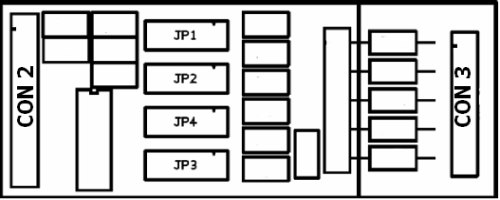
\includegraphics[width=0.50\textwidth,bb=0 0 500 200]{images/108.png}
	\caption{[FLEX108] Details of FLEX Multibus Serial TTL Module}
	\label{fig:108detail}
\end{figure}

\begin{small}
\begin{table}[!ht]
\centering
\begin{tabular}{|c|c|c|}
	\hline
	{\bf Jumper} & {\bf pos. 1-2} & {\bf pos. 2-3}\\
	\hline
	JP1 & TX\_1 & GND\\
	\hline
  JP2 & SCK\_1 & GND\\
	\hline
  JP3 & TX\_TTL & GND\\
	\hline
  JP4 & RTS\_TTL & GND\\
	\hline
  \multicolumn{3}{l}{\begin{tiny}Note: Default jumper settings are indicated by a $\bullet$\end{tiny}}\\
\end{tabular}
\caption{FLEX108 - Jumpers}
\label{tbl:108jps}
\end{table}
\end{small}

\begin{small}
\begin{table}[!ht]
\centering
\begin{tabular}{|c|l|}
	\hline
	Pin 1 & +5V\\
	\hline
  Pin 2 & TX\_1\\
	\hline
  Pin 3 & SCK\_1\\
	\hline
  Pin 4 & RX\_1\\
	\hline
  Pin 5 & FRCK\_1\\
	\hline
  Pin 6 & GND\\
	\hline
\end{tabular}
\caption{FLEX108 - CON2}
\label{tbl:108con2}
\end{table}
\end{small}

\begin{small}
\begin{table}[!ht]
\centering
\begin{tabular}{|c|l|}
	\hline
	Pin 1 & CTS\_TTL\\
	\hline
  Pin 2 & RX\_TTL\\
	\hline
  Pin 3 & TX\_TTL\\
	\hline
  Pin 4 & RTS\_TTL\\
	\hline
  Pin 5 & GND\\
	\hline
\end{tabular}
\caption{FLEX108 - CON3}
\label{tbl:108con3}
\end{table}
\end{small}
%|||||||||||||||||||||||||||||||||||||||||||||||||||||||||
%+-+-+-+-+-+-+-+-+-+-+-+-+-+-+-+-+-+-+-+-+-+-+-+-+-+-+-+-+-+-+-+-+
\clearpage
\subsection{Multibus I2C Module}
\label{subsec:i2c}
%+-+-+-+-+-+-+-+-+-+-+-+-+-+-+-+-+-+-+-+-+-+-+-+-+-+-+-+-+-+-+-+-+
The I2C Module fits on slot 5 of the FLEX Multibus Base Daughter Board, refer Figure ~\ref{fig:101detail}.\\
\noindent This module can be used to connect in a safe way an I2C bus to one of the I2C peripherals of the dsPIC�. The protection includes protection from spikes, as well as hot insertions and hot extractions.\\
%|||||||||||||||||||||||||||||||||||||||||||||||||||||||||




%+-+-+-+-+-+-+-+-+-+-+-+-+-+-+-+-+-+-+-+-+-+-+-+-+-+-+-+-+-+-+-+-+
\clearpage
\subsection{[FLEX109] FLEX Demo Daughter Board}
\label{subsec:109}
%+-+-+-+-+-+-+-+-+-+-+-+-+-+-+-+-+-+-+-+-+-+-+-+-+-+-+-+-+-+-+-+-+
The FLEX Demo Board, as depicted in Figures ~\ref{fig:109a} and ~\ref{fig:109b}, is a FLEX Daughter Board, refer Section ~\ref{sec:daughter}, targeted specifically for educational institutions e.g. Schools and Universities.\\

\begin{figure}[!ht]
	\centering
		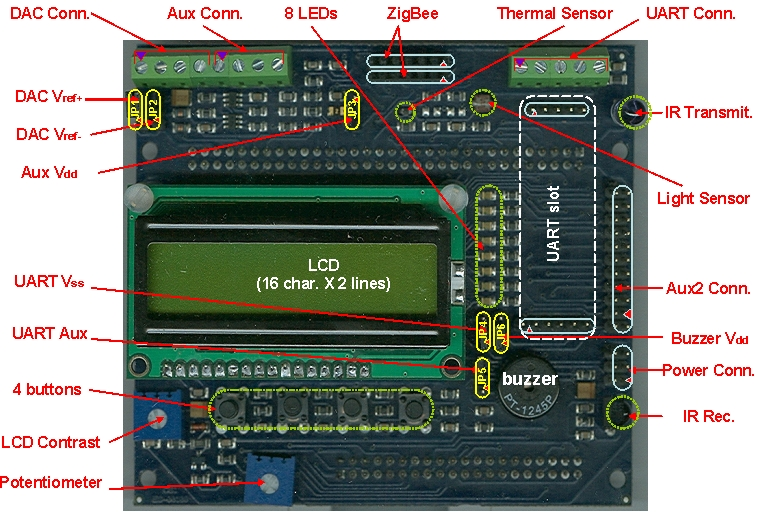
\includegraphics[width=0.90\textwidth,bb=0 0 758 512]{images/flex109a.jpg}
	\caption{[FLEX109] FLEX Demo Daughter Board - front side}
	\label{fig:109a}
\end{figure}
\begin{figure}[!ht]
	\centering
		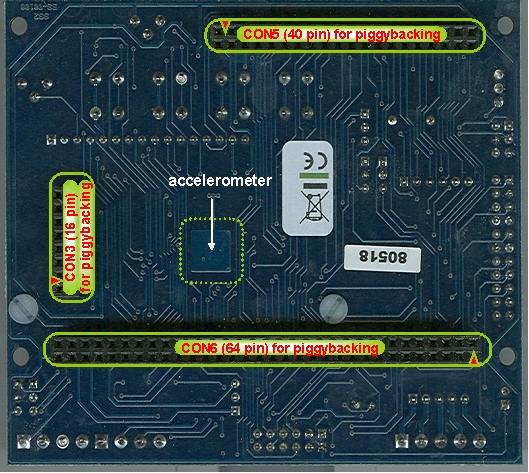
\includegraphics[width=0.90\textwidth,bb=0 0 529 473]{images/flex109b.jpg}
	\caption{[FLEX109] FLEX Demo Daughter Board - back side}
	\label{fig:109b}
\end{figure}

\noindent The FLEX Demo Board fits directly on FLEX Base Boards (FLEX Full, refer Subsection ~\ref{subsec:001}/FLEX Light, refer Subsection ~\ref{subsec:003}) and it adds-on a lot of most commonly used features that are used for carrying out prototyping and laboratory experiments.\\

\noindent The features hosted on Demo Board are:
\begin{itemize}
  \item 2 DAC outputs (12 bit resolution)
  \item 3-axis accelerometer (selectable range from 1.5g to 6g)
  \item Direct support for quadrature encoder
  \item Set of 4 Push buttons
  \item Set of 8 LEDs
  \item LCD (16 characters x 2 lines)
  \item Buzzer
  \item Potentiometer
  \item Thermal sensor
  \item Light sensor
  \item InfraRed receiver and transmitter
  \item ZigBee connector
  \item Socket for Multibus serial modules (one of FLEX103, FLEX104, FLEX105, and FLEX108)
  \item USB wiring for FLEX Full Base Board
\end{itemize}

\noindent {\tt Note: The FLEX Demo Board is fully supported by Scilab/Scicos code generator, where specific blocks are available to directly control the main peripherals. Hence, applications can be entirely generated without writing any C code!}\\


%^^^^^^^^^^^^^^^^^^^^^^^^^^^^^^^^^^^^^^^^^^^^^^^^^^
\subsubsection{Technical details}
\label{subsubsec:109tech}
%^^^^^^^^^^^^^^^^^^^^^^^^^^^^^^^^^^^^^^^^^^^^^^^^^^
\begin{figure}[!ht]
	\centering
		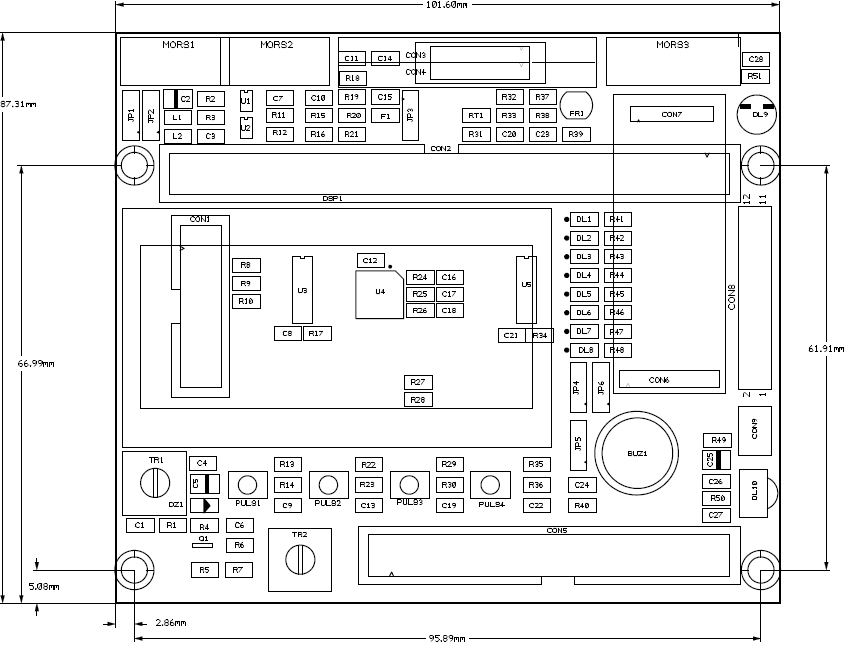
\includegraphics[width=0.90\textwidth,bb=0 0 845 645]{images/109mec.png}
	\caption{[FLEX109] Dimensions of FLEX Demo Daughter Board}
	\label{fig:109mec}
\end{figure}
\begin{figure}[!ht]
	\centering
		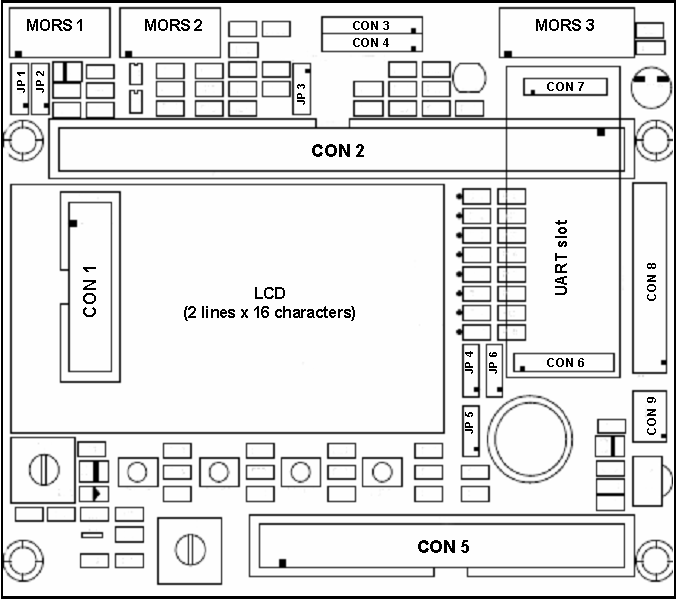
\includegraphics[width=0.90\textwidth,bb=0 0 677 599]{images/109.png}
	\caption{[FLEX109] Details of FLEX Demo Daughter Board}
	\label{fig:109detail}
\end{figure}

\begin{small}
\begin{table}[!ht]
\centering
\begin{tabular}{|c|l|}
  \hline
  Pin 1 & Analog Output 1\\
	\hline
	Pin 2 & GND \\
	\hline
	Pin 3 & Analog Output 2\\
	\hline
	Pin 4 & GND \\
	\hline
\end{tabular}
\caption{FLEX109 - MORS1 (DAC Connector)}
\label{tbl:109mors1}
\end{table}
\end{small}

\begin{small}
\begin{table}[!ht]
\centering
\begin{tabular}{|c|l|}
  \hline
	Pin 1 & Data 1\\
	\hline
	Pin 2 & Data 2\\
	\hline
	Pin 3 & Vout/+5V (selectable)\\
	\hline
	Pin 4 & GND\\
	\hline
\end{tabular}
\caption{FLEX109 - MORS2 (AUX Connector)}
\label{tbl:109mors2}
\end{table}
\end{small}

\begin{small}
\begin{table}[!ht]
\centering
\begin{tabular}{|c|l|}
  \hline
	Pin 1 & CTS (232/TTL)/TX+ (422)\\
	\hline
	Pin 2 & RX (232/TTL)/TX- (422)/485- (485)\\
	\hline
	Pin 3 & TX (232/TTL)/RX+ (422)/485+ (485)\\
	\hline
	Pin 4 & RTS (232/TTL)/RX- (422)\\
	\hline
	Pin 5 & GND\\
	\hline
\end{tabular}
\caption{FLEX109 - MORS3 (UART Connector)}
\label{tbl:109mors3}
\end{table}
\end{small}

\begin{small}
\begin{table}[!ht]
\centering
\begin{tabular}{|l|l|}
  \hline
	DL1 (yellow) & RF0\\
	\hline
	DL2 (yellow) & RF1\\
	\hline
	DL3 (yellow) & RF2\\
	\hline
	DL4 (yellow) & RF3\\
	\hline
	DL5 (yellow) & RD8\\
	\hline
	DL6 (yellow) & RD9\\
	\hline
	DL7 (yellow) & RD10\\
	\hline
	DL8 (yellow) & RD11\\
	\hline
\end{tabular}
\caption{FLEX109 - LEDs}
\label{tbl:109leds}
\end{table}
\end{small}


\begin{small}
\begin{table}[!ht]
\centering
\begin{tabular}{|l|c|c|}
  \hline
  {\bf Jumper} & {\bf pos. 1-2} & {\bf pos. 2-3}\\
  \hline
	[JP1] DAC Vref+ & $\bullet$ +5V & +3.3V\\
	\hline
	[JP2] DAC Vref- & $\bullet$ GND & GNDout\\
	\hline
	[JP3] Aux Vdd & $\bullet$ Vout & +5V\\
	\hline
	[JP4] UART Vss & $\bullet$ GND & GNDout\\
	\hline
	[JP5] UART Aux & INT (Konnex/EIB) & $\bullet$ RTS (232/422/TTL)\\
	\hline
	[JP6] Buzzer Vdd & $\bullet$ Vout & +5V\\
	\hline
  \multicolumn{3}{l}{\begin{tiny}Note: Default jumper settings are indicated by a $\bullet$\end{tiny}}\\
\end{tabular}
\caption{FLEX109 - Jumpers}
\label{tbl:109jps}
\end{table}
\end{small}

\begin{small}
\begin{table}[!ht]
\centering
\begin{tabular}{|c|c|c|c|}
  \hline
	{\bf Push Btn.} & {\bf pin} & {\bf pos. 1-2 (normal)} & {\bf pos. 2-3 (pressed)}\\
	\hline
	PULS1 & RD4 & +5V & GND\\
	\hline
	PULS2 & RD5 & +5V & GND\\
	\hline
	PULS3 & RD6 & +5V & GND\\
	\hline
	PULS4 & RD15 & +5V & GND\\
	\hline
\end{tabular}
\caption{FLEX109 - Push Buttons}
\label{tbl:109btns}
\end{table}
\end{small}

\begin{small}
\begin{table}[!ht]
\centering
\begin{tabular}{|l|l||l|l|}
  \hline
	\multicolumn{2}{|c||}{\bf CON3} & \multicolumn{2}{c|}{\bf CON4}\\
	\hline
	Pin 1 & +3.3V & Pin 1 & GND\\
	\hline
	Pin 2 & Reset & Pin 2 & Vreg\\
	\hline
	Pin 3 & FIFO & Pin 3 & CSN\\
	\hline
	Pin 4 & SDO & Pin 4 & SDI\\
	\hline
	Pin 5 & SCK & Pin 5 & CCA\\
	\hline
	Pin 6 & SFD & Pin 6 & FIFOP\\
	\hline
\end{tabular}
\caption{FLEX109 - CON3+CON4 (ZigBee Connector)}
\label{tbl:109con3con4}
\end{table}
\end{small}

\begin{small}
\begin{table}[!ht]
\centering
\begin{tabular}{|c|l|}
	\hline
	Pin 1 & +5V\\
	\hline
	Pin 2 & RF5 (TX1)\\
	\hline
	Pin 3 & RF12 (SCK1)\\
	\hline
	Pin 4 & RF4 (RX1)\\
	\hline
	Pin 5 & JP6 (default pos. 1-2 i.e. Vout)\\
	\hline
	Pin 6 & JP4 (default pos. 2.3 i.e. GND)\\
	\hline
\end{tabular}
\caption{FLEX109 - CON6 (Connected to Serial TTL)}
\label{tbl:109con6}
\end{table}
\end{small}

\begin{small}
\begin{table}[!ht]
\centering
\begin{tabular}{|c|l|}
	\hline
	Pin 1 & CTS (232/TTL)/TX+ (422)\\
	\hline
	Pin 2 & RX (232/TTL)/TX- (422)/485- (485)\\
	\hline
	Pin 3 & TX (232/TTL)/RX+ (422)/485+ (485)\\
	\hline
	Pin 4 & RTS (232/TTL)/RX- (422)\\
	\hline
	Pin 5 & GND\\
	\hline
\end{tabular}
\caption{FLEX109 - CON7 (connected to MORS3)}
\label{tbl:109con7}
\end{table}
\end{small}

\begin{small}
\begin{table}[!ht]
\centering
\begin{tabular}{|l|l||l|l|}
	\hline
	Pin 1 & Encoder Index & Pin 2 & PWMout 1L\\
	\hline
	Pin 3 & Encoder Channel A & Pin 4 & PWMout 1H\\
	\hline
	Pin 5 & Encoder Channel B & Pin 6 & PWMout 2L\\
	\hline
	Pin 7 & OC8 & Pin 8 & PWMout 2H\\
	\hline
	Pin 9 & Analog Input 19 & Pin 10 & PWMout 3L\\
	\hline
	Pin 11 & OC3 & Pin 12 & PWMout 3H\\
	\hline
	Pin 13 & DSPPCLK & Pin 14 & PWMout 4L\\
	\hline
	Pin 15 & DSPPDATA & Pin 16 & PWMout 4H\\
	\hline
	Pin 17 & DSPMCLR & Pin 18 & Analog Input 20\\
	\hline
	Pin 19 & AV SSext & Pin 20 & Analog Input 21\\
	\hline
	Pin 21 & AV DDext & Pin 22 & GND\\
	\hline
\end{tabular}
\caption{FLEX109 - CON8 (AUX2 Connector)}
\label{tb1:109con8}
\end{table}
\end{small}

\begin{small}
\begin{table}[!ht]
\centering
\begin{tabular}{|c|l|}
	\hline
	Pin 1 & Vout\\
	\hline
	Pin 2 & GNDout\\
	\hline
	Pin 3 & +5V\\
	\hline
	Pin 4 & GND\\
	\hline
	Pin 5 & +3.3V\\
	\hline
	Pin 6 & GND\\
	\hline
\end{tabular}
\caption{FLEX109 - CON9 (Power Connector)}
\label{tbl:109con9}
\end{table}
\end{small}